\section{Nube de Conductores}\label{section:NubeConductores}
El núcleo del sistema es una aplicación desplegada en la nube, la cual se ha denominado \emph{Nube de Conductores}, donde se concentran en una base de datos la información relativa a ciclistas y vehículos a motor. Un servicio de aplicación web embebido llamado \emph{Jetty} se encarga de recibir y atender los mensajes \Gls{http/1.1} que son enviados desde la parte de vehículos a motor y ciclistas. Dos \emph{Handler} independientes se encargan de filtrar los mensajes que no han sido correctamente construidos, es decir, tienen un formato inválido, e insertar y actualizar los datos de la base de datos.

Para el despliegue de la aplicación se utilizado una máquina virtual \emph{Ubuntu Server 14.04 LTS} que cuenta con 2048 MiB de memoria RAM y 2 núcleos para procesamiento. También se ha reservado un dominio público para que las peticiones puedan ser enviadas al servidor. Gracias a la herramienta Ant se puede cambiar fácilmente la plataforma donde se distribuya la aplicación, además esta configurada para poder ser ejecutada directamente con el comando \emph{run}.

Como puede observarse en la figura \ref{fig:DiagComponentes-Nube} los clientes acceden a la nube a través de dos gestores independientes a través de mensajes \gls{http/1.1}. Los datos son almacenados en \emph{Hash Map} para acceder directamente a los datos. Estos datos son empleados por el calculador de alertas para predecir si dos vehículos pueden colisionarse; en caso de que pueda suceder, se emplea el emisor de alertas para enviar un mensaje a través de \gls{http/1.1} al cliente correspondiente.

\begin{figure}[H]
	\begin{center}
		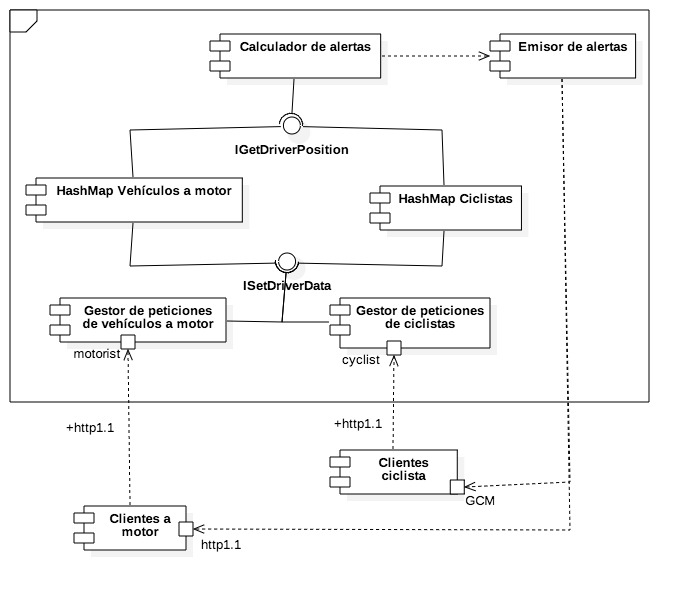
\includegraphics[scale=0.4]{DiagComponentes-Nube}
		\caption{Arquitectura de la Nube de Conductores}
		\label{fig:DiagComponentes-Nube}
	\end{center}
\end{figure}

\subsection{Procesos}\label{ssection:procesos}
A través del \gls{api} de Jetty la aplicación crea un servidor con dos \emph{handler} de mensajes, uno para ciclistas y otro para vehículos a motor. A través de ellos la Nube de Conductores recibe datos de ciclistas y vehículos a motor, almacenándolos en una base de datos interna sin necesidad de utilizar un DBMS, ya que no hace falta que los datos sean persistentes más tiempo de lo que los vehículos estén emitiendo su posición. Cada manejador posee un \emph{ThreadPool} con el que crea un gestor para cada mensaje recibido, este esta limitado a un número de hilos para evitar que la aplicación se colapse.

Un registro se considera antiguo cuando no ha sido refrescado en un período de un minuto. Para evitar que emplee información obsoleta, se ejecuta una rutina que tan solo mantiene en memoria los registros que periódicamente están siendo actualizados; esto se realiza gracias al campo de \emph{timestamp}.

Paralelamente, cada vez que un mensaje es recibido en uno de los \emph{handler} (conductores o ciclistas), otro algoritmo compara la posición obtenida a través del handler con la de los vehículos existentes. Si se detecta que algún ciclista o vehículo a motor están próximos 
- en un rango menor a 200 metros - se manda a ambos vehículos una alerta avisándoles de su proximidad \emph{[Algoritmo \ref{alg:proximidadVehiculos}]}. En la sección \ref{ssection:algPrediccion}, se detalla el funcionamiento del algoritmo que se encarga de predecir si dos vehículos pueden encontrarse.

\begin{listing}
	\begin{minipage}{.4\textwidth}
		\begin{minted}[linenos=true]{java}
for (Motorist m : lMotorist) {
  for (Cyclist c : lCyclist) {
    if (isCollisionDanger(m, c)) {
      sendWarningToMotorist(c);
      sendCyclistPositionToMotorist(c);
    }
  }
}
		\end{minted}
	\end{minipage}
	\caption{Cálculo de la proximidad de los vehículos}\label{alg:proximidadVehiculos}
\end{listing}

\subsection{Algoritmos de predicción}\label{ssection:algPrediccion}
\subsubsection{Posición vehicular relativa}
La posición vehicular relativa se refiere a en qué lado de un vehículo A se encuentra un vehículo B. Es decir, si se toma como referencia el primer vehículo, en qué lado se encuentra el segundo; derecha, izquierda, delante o detrás.

El sistema de coordenadas GPS emplea un sistema diferente del cartesiano; el ángulo 0 comienza donde en el sistema tradicional (cartesiano) serían 90º. Además, en vez de ir aumentando los grados de forma antihoraria lo hace al contrario, es decir, aumenta los grados en sentido horario [Figura \ref{figure:rumbo_gps}].

El heading representa la dirección hacia la que un vehículo se está moviendo, empleando el norte (0º) como referencia. Esta información, junto con la latitud, longitud y altitud (Alt.) de los ciclistas y vehículos, es obtenida a través del GPS. Primero, se calcula el ángulo existente entre los dos vehículos tomando como referencia al ciclista, con esto se obtiene la posición del vehículo sin tener en cuenta la dirección hacia la que circula el ciclista. Seguidamente, se relacionan el heading del ciclista y el ángulo entre los dos vehículos para obtener el ángulo relativo entre ambos. Es decir, el ángulo respecto la posición y dirección del ciclista, y la posición del vehículo. Finalmente, si el ángulo relativo se encuentra entre 15º y 345º, se considera que está delante; entre 120º y 230º, se encuentra detrás de su posición; entre 15º y 120º se considera que está a su derecha; y entre 230º y 345º, a su izquierda. Estos cálculos son realizados en cada vehículo. En la figura \ref{figure:demo_pos_relativa} se muestra un ejemplo del funcionamiento del algoritmo en un entorno real.

El funcionamiento del algoritmo \ref{alg:relative_vehicular_pos} se puede resumir de la siguiente forma:
\begin{enumerate}
	\item Calcular el ángulo existente entre los dos vehículos, sin tener en cuenta la dirección del primer vehículo.
	\item Se resta el heading del vehículo de referencia, al ángulo que hay entre los dos vehículos.
	\item Se contrasta con una serie de casos ya conocidos, y se devuelve el ángulo	relativo.
\end{enumerate}

\begin{listing}
	\begin{minipage}{.4\textwidth}
		\begin{minted}[linenos=true]{javascript}
function calcularPosicionRelativa(heading, oLatitude, oLongitude, pLatitude, pLongitude) {
  var degrees = calculateAngleBetweenTwoPoints(oLatitude, oLongitude, pLatitude, pLongitude);
  var relativeAngle = correctDegrees(degrees - heading);
				
  if (relativeAngle <= 15 && >= 0 || relativeAngle >= 345 && relativeAngle < 360)
    return "FRONT";
  else if (relativeAngle >= 120 && relativeAngle <= 230)
    return "BACK";
  else if (relativeAngle < 120 && relativeAngle > 15)
    return "RIGHT";
  else
    return "LEFT";
}

function calcularAnguloEntreDosPuntos(ox, oy, x, y) {
  return toDegrees(Math.atan2(y - oy, x - ox));
}
\end{minted}
\end{minipage}
\caption{Cálculo de la posición relativa vehicular.}\label{alg:relative_vehicular_pos}
\end{listing}

\begin{figure}[h]
	\begin{center}
		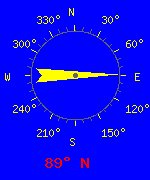
\includegraphics[scale=0.7]{bearing-1427303542791}
		\caption{Rumbo: el ángulo 0º está desplazado 90º con respecto al eje cartesiano.}
		\label{figure:rumbo_gps}
	\end{center}
\end{figure}
\begin{figure}[h]
	\begin{center}
		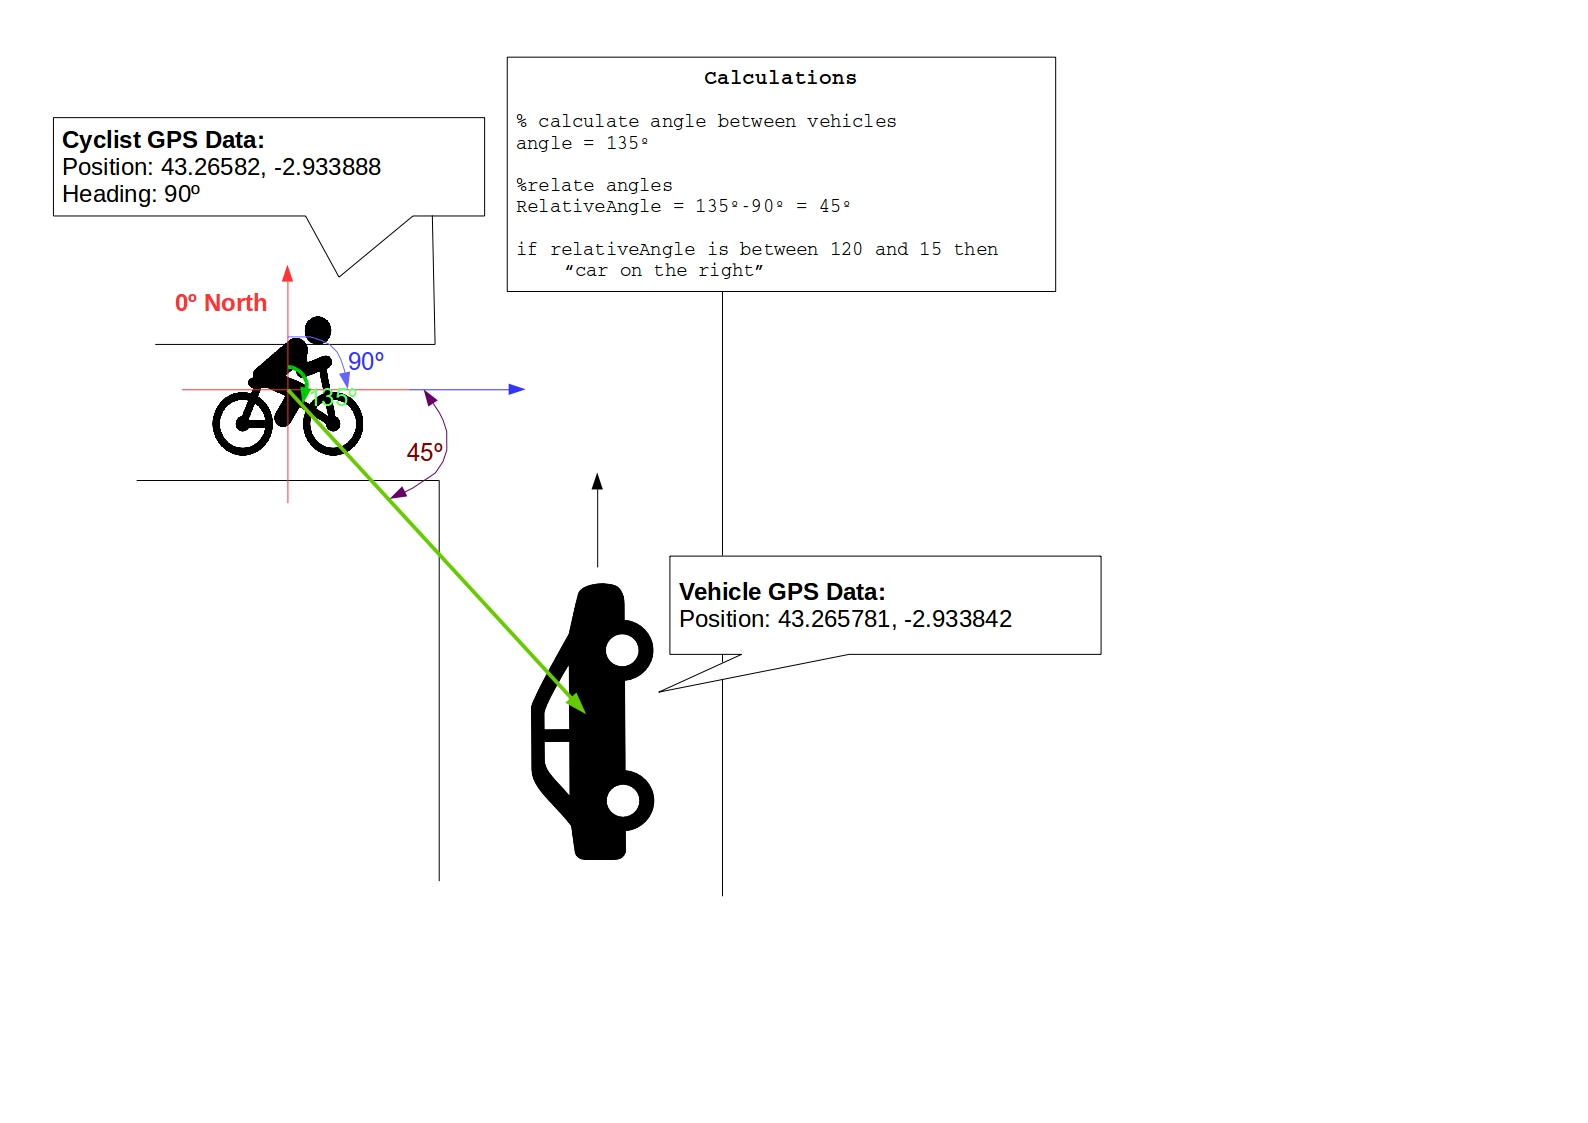
\includegraphics[scale=0.3]{demo-pos-relativa}
		\caption{Posición relativa vehicular.}
		\label{figure:demo_pos_relativa}
	\end{center}
\end{figure}
\subsubsection{Previsor de accidentes}
El algoritmo de posición vehicular relativa por sí solo no es suficiente para detectar cuándo dos vehículos pueden encontrarse, tan solo prevé por dónde se puede encontrar un vehículo. Por lo que para detectar una posible colisión es necesario un algoritmo que emplee la posición vehicular relativa, la distancia entre los dos vehículos y el sentido en que circulan ambos.

Mediante el algoritmo \ref{alg:deteccion_colisiones} se detecta si dos vehículos pueden cruzarse en un rango de distancia especificado. Para ello, se requiere la posición de ambos vehículos y la dirección hacia la que circulan. Se aplica un algoritmo para calcular la nueva posición de ambos vehículos en el rango de distancia que se desee. Con las cuatro posiciones obtenidas, primero se calcula si existe un punto de intersección, entre las dos rectas. Finalmente, se comprueba si las rectas cortan entre las posiciones hacia la que se dirigen los vehículos.
\FloatBarrier